\documentclass{article}
\usepackage{graphicx} % Required for inserting images
\usepackage{minted}

\title{Root Finding Algorithms}
\author{Alex Zhou}
\date{April 2019}

\begin{document}

\maketitle

\section{Introduction}

We consider four iterative methods to find a numerical solution of an algebraic or transcendental equation \(F(x) = 0\) in one dimension, in particular, those without a closed form solution. We want to compute a sequence \(x_0, x_1, x_2, \dots\) such that
\[ \lim_{n \to \infty} x_n = x_* \quad \mbox{where} \quad f(x_*) = 0. \]

\begin{enumerate}
    \item Interval bisection, also known as binary search which involves successively halving the search space at each iteration by evaluating the function at the midpoint \(d = \frac{x_0 + x_2}{2}\).
    \item Secant method, which interpolates between two points and their values iteratively to compute the 2nd order recurrence
    \[  x_{n+1} = x_n - \frac{x_n - x_{n-1}}{f(x_n) - f(x_{n-1})}f(x_n). \]
    \item Fixed point iteration, where we consider the equivalent system \(x = f(x)\), (which is not necessarily unique), and then apply the iteration scheme, \(x_{n+1} = f(x_{n})\).
    \item Newton-Raphson iteration, which uses the derivative to solve the 1st order iteration scheme
    \[ x_{n+1} = \frac{F(x_{n})}{F'(x_{n})}. \]
\end{enumerate}

For each of these methods, we shall also consider the order of convergence. A sequence \(\delta_n\) which converges to zero as \(n \to \infty\) is said to have order of convergence \(p \geq 1\) if
\[ \lim_{n \to \infty} \frac{|\delta_n|}{|\delta_{n-1}|^p} = C \]
for some \(C > 0\). If a method is convergent, \(\epsilon_n = x_n - x_* \to 0\) as \(n \to \infty\), then it is said to be \(p\)th-order convergent if either \((\epsilon_n)\) has order of convergence \(p\) or if it is dominated by a sequence which has order of convergence \(p\).

\section{Interval Bisection}
The idea of interval bisection is to find two points \(a, b\) satisfying \(F(a)F(b) < 0\), that is, \(F(a)\) and \(F(b)\) have opposite signs. Therefore, by the intermediate value theorem, we can find a root of \(F\) in the interval \((a, b)\). We repeat this process by swapping out the endpoint whose function value has the same sign as the midpoint \(d = \frac{a + b}{2}\). It is clear that \(\frac{\epsilon_n}{\epsilon_{n-1}} = \frac{1}{2}\), giving first-order convergence. The following is an implementation in Python:

\begin{minted}[linenos, autogobble]{python}
    import numpy as np
        
    def bisection(func, a, b, tol, err, step = 0):
        if a >= b:
            raise Exception("Lower bound is greater than upper bound")
        if tol < 0 or err < 0:
            raise Exception("Negative tolerance or error")
        if np.sign(func(a)) == np.sign(func(b)):
            raise Exception("No root found")
            
        # Compute the midpoint between a and b
        mid = (a + b) / 2
        step = step + 1
        if np.abs(func(mid)) < err or np.abs(a - b) < 2 * tol:
            # Found root within tolerance or error
            return mid, func(mid), step
        elif np.sign(func(a)) == np.sign(func(mid)):
            # mid improves a, recursively call
            return bisection(func, mid, b, tol, err, step)
        elif np.sign(func(b)) == np.sign(func(mid)):
            # mid improves b, recursively call
            return bisection(func, a, mid, tol, err, step)
\end{minted}

Consider the function \(F(x) = 2x - 3\sin(x) + 5\). Note that for \(x < -4\), we have \(2x + 5 < -3 \leq -3|\sin(x)|\), whilst for \(x > - 1\), we have \(2x + 5 > 3 \geq 3|\sin(x)|\), hence there are no roots of \(f\) that lie outside the interval \([-4, -1]\). Note that in the intervals \([-4, -\pi]\) and \([-5/2, -1]\), the functions \(2x + 5\) and \(-3\sin(x)\) have the same signs, so their sum can never vanish. 

\begin{figure}
    \centering
    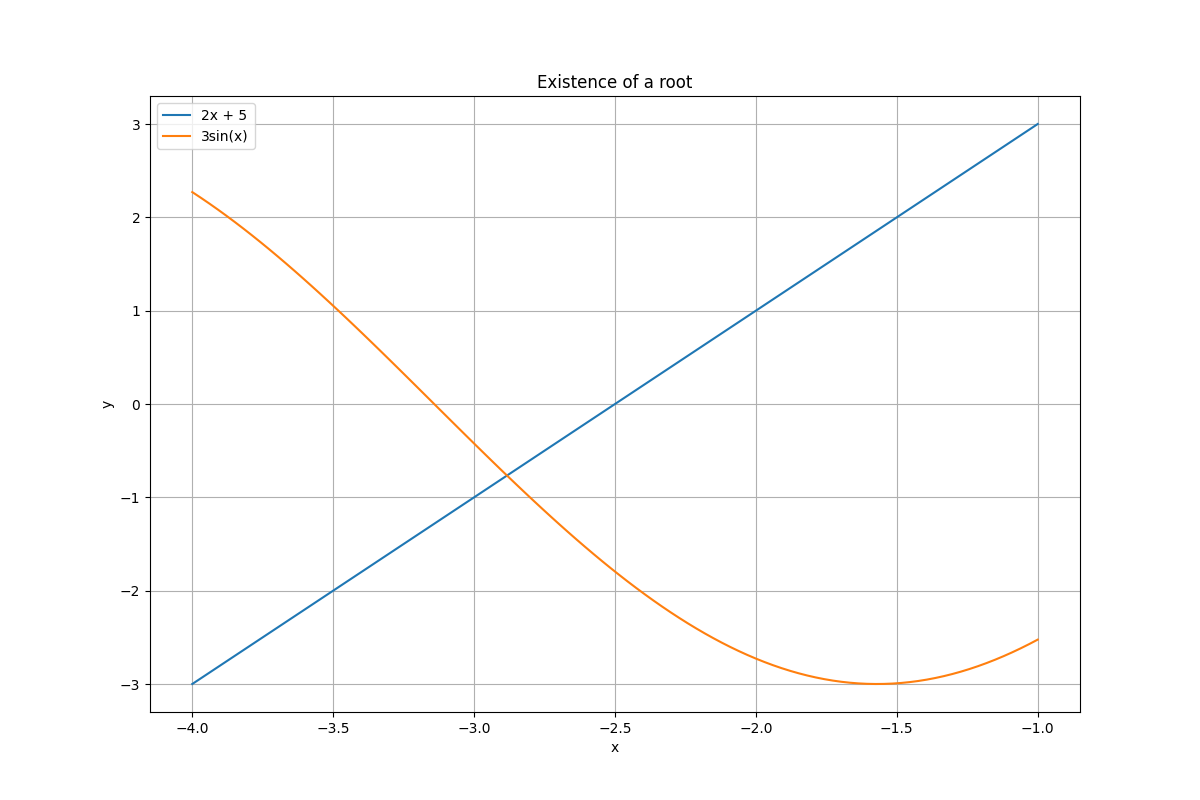
\includegraphics[width=1.0\linewidth]{root_intersect.png}
    \caption{Plot of \(2x+5\) and \(3\sin(x)\).}
\end{figure}

The remaining interval to consider is \([-\pi, -5/2]\), where \(2x + 5\) is increasing to \(0\) and \(-3\sin(x)\) is increasing from \(0\) as \(-5/2 < -\pi/2\), yielding exactly one intersection point which is a root of \(F\). Running these starting values for our bisection algorithm with tolerance \(0.5 \cdot 10^{-5}\) yields:

\begin{verbatim}[Output]
    F = lambda x: 2 * x - 3 * np.sin(x) + 5
    bisection(F, -np.pi, -5/2, 0.5*10**(-5), 0)
    (-2.8832413759422737, -2.2068544265785306e-05, 17)
\end{verbatim}

Of course, there is a rounding error when evaluating \(F\) using a computer. Let this rounding error be at most \(\delta\) for \(|x| < \pi\) and consider the final interval \([a,b]\) of our bisection. Then, \(F(a)\) and \(F(b)\) have opposite signs and have magnitude less than \(\delta\). Consider a Taylor expansion of \(F\) about the approximation \(x_*\),
\[ F(x) = F'(x)(x - x_*) + O((x - x_*)), \]
therefore
\[ |x - x_*| \approx \left| \frac{F(x)}{F'(x_*)} \right| \leq \frac{\delta}{|F'(x_*)|}. \]
Setting the midpoint \(x_* = \frac{a+b}{2}\) such that the actual value of \(x_*\) has error bounded by \(\frac{b-a}{2}\), we obtain the error bound
\[ x_* = \frac{a+b}{2} \leq \frac{b-a}{2} + \frac{\delta}{|F'(x_*)|}. \]
Using the fact that \(|F'(x)| > 4\) for \(x \in (-5\pi/4, -3\pi/4)\), if the bisection algorithm is terminated when \(\frac{b-a}{2} < 0.5 \cdot 10^{-5}\), then the error is bounded by \(0.5 \cdot 10^{-5} + \frac{\delta}{4}\).

\section{Secant Interpolation}
Given two points \(x_0\) and \(x_1\), not necessarily with opposite signs, we iterate the secant line between the two points on the function \(F\),
\[ x_{n+1} = x_n - \frac{x_n - x_{n-1}}{F(x_n) - F(x_{n-1})}F(x_n). \]
We can see the secant method also as a finite difference approximation of the Newton-Raphson method which we will explore later.

Unlike bisection, the resulting sequence is not guaranteed to converge to a root of \(F\), however convergence can be faster, typically of order \(\varphi\) (the golden ratio) which is super-linear but sub-quadratic. Similar to bisection, prior information (initial interval) can be helpful, especially to guarantee convergence.

Compared to the Newton-Raphson method or a fixed-point iterative method, we do not require any computation of the derivative, but we do need to keep track of two points rather than one.

\section{Fixed-Point Iteration}
To solve \(F(x) = 0\), we first rewrite this as \(x = f(x)\) (not necessarily uniquely). Choose an initial \(x_0\) and iterate \(x_n = f(x_{n-1})\). If \(F(x_*) = 0\), then \(f(x_*) = x\), so fixed points of \(f\) can be used to find the roots of \(F\). One such choice of function is \(f(x) = x - h(F(x))\) for some functional \(h\) satisfying \(h(0) = 0\). An implementation of this in Python is written below:

\begin{minted}[linenos, autogobble]{python}
    import numpy as np
    
    def picard_iteration(guess, func, tol, err, max_steps, h):
        x0 = guess
        for i in range(1, max_steps + 1):
            x1 = x0 - h(func(x0))
            print((x1, func(x1), i))
            if np.abs(x1 - x0) <= tol or np.abs(func(x1)) <= err:
                break
            x0 = x1
        return x1, func(x1), i
\end{minted}

Setting \(h = \frac{F}{2 + k}\) so that 
\[f(x) = \frac{3\sin(x) + kx - 5}{2 + k}. \]
Running this program for \(k = 0\), tolerance \(10^{-5}\) and starting point \(x_0 = -2\) for \(10\) steps gives a two-point oscillation which does not converge to the root.

\begin{verbatim}[Output]
    F = lambda x: 2 * x - 3 * np.sin(x) + 5
    k = 0
    h = lambda y: y / (2 + k)
    picard_iteration(-2, F, 10**-5, 0, 10, h)
    (-3.8639461402385225,   -4.71134890733369,      1)
    (-1.5082716865716774,   4.977594541013409,      2)
    (-3.997068957078382,    -5.258788083242857,     3)
    (-1.3676749154569534,   5.20297519604766,       4)
    (-3.9691625134807835,   -5.1471924803077584,    5)
    (-1.3955662733269043,   5.162926829345091,      6)
    (-3.97702968799945,     -5.178828681999924,     7)
    (-1.3876153469994876,   5.174576986162576,      8)
    (-3.9749038400807755,   -5.170293563781206,     9)
    (-1.3897570581901726,   5.171457188695995,      10)
\end{verbatim}

We can explain this divergence as follows. For \(x_n\) close to the root \(x_*\), we have the recurrence
\[ x_n = f(x_{n-1}) \approx f(x_*) + f'(x_*)(x_{n-1} - x_*) = x_* + f'(x_*)(x_{n-1} -x_*), \]
so the truncation error \(\epsilon_n = |x_n - x_*|\) satisfies the difference equation
\[ \epsilon_n \approx f'(x_*) \epsilon_{n-1}. \]
Thus, this iteration scheme will diverge whenever \(|f'(x_n)| > 1\) which is indeed the case at the root \(x_*\) by considering the derivative
\[ f'(x) = \frac{3\cos(x) + k}{2 + k}, \]
for \(k = 0\). Conversely, we may obtain convergence if \(|f'(x_*)| < 1\). To see this, apply the mean value theorem on the interval bounded by \(x_*\) and \(x_{n-1}\),
\[ x_n - x_* = f(x_{n-1}) - f(x_*) = f'(\xi)(x_{n-1} -x_*), \]
for some \(\xi\) in the interval. If \(x_{n-1}\) also lies in the same interval, and \(|f')(\xi)| < 1\), this proves that \(f\) is a contraction mapping and the iteration scheme converges to a unique fixed point. 

In the range \([-\pi, -\pi/2]\), we have the bound
\[ |f'(\xi)| = \left|\frac{3\cos(\xi) + k}{2 + k}\right| < 1, \]
for all \(\xi \in [-\pi, -\pi/2]\) whenever \(k < \frac{1}{2}\). Thus, convergence is guaranteed if \(k< \frac{1}{2}\) and \(x_0 \in [-\pi, -\pi/2]\). Observe that the denominator of the derivative is negative for \(k < 3\) (approximately) and is positive for \(k >  3\). These values of \(k\) give us oscillatory and monotonic convergence respectively, and taking \(k\) close as possible to \(3\) so that \(|f'(\xi)|\) is small should give us rapid convergence. Taking \(k - 2.5\) yields:

\begin{verbatim}[Output, oscillatory convergence]
    (-2.8284205067726766,   0.26739310181149367,        1)
    (-2.8878411960641195,   -0.02257126128216491,       2)
    (-2.8828253602236384,   0.0020165241474270346,      3)
    (-2.8832734767008446,   -0.00017937670205547818,    4)
    (-2.883233615211499,    1.5962409209535622e-05,     5)
    (-2.8832371624135456,   -1.4204166438602783e-06,    6)
\end{verbatim}

whilst taking \(k - 3.5\):

\begin{verbatim}[Output, monotonic convergence]
    (-2.677798596450372,    0.9864365408023481,         1)
    (-2.8571506947780714,   0.12756424089329688,        2)
    (-2.880344193122307,    0.014172166494031302,       3)
    (-2.8829209506666764,   0.0015481161473527294,      4)
    (-2.8832024263298313,   0.0001688010179528021,      5)
    (-2.8832331174240045,   1.8401782686083834e-05,     6)
    (-2.8832364632026746,   2.006020123346275e-06,      7)
\end{verbatim}

To demonstrate slower convergence, we take \(k = 16\):

\begin{verbatim}[Output, slow convergence]
    (-2.207105126693169,    2.998673716107927,          1)
    (-2.3736981109213873,   2.336470277643329,          2)
    (-2.5035020152349055,   1.7799845580235774,         3)
    (-2.6023900462362155,   1.335575600559979,          4)
    ...
    (-2.883182169855864,    0.0002680658417055781,      31)
    (-2.8831970624026257,   0.00019508643711230178,     32)
    (-2.8832079005380207,   0.00014197515449776432,     33)
    (-2.883215788046604,    0.0001033230897498072,      34)
\end{verbatim}

Note that rearranging the recurrence yields
\[ x_n - x_{n-1} \approx (f'(x_{n-1}) - 1)(x_{n-1} - x_*) \approx  (f'(x_{n-1}) - 1) \frac{x_n - x_*}{f'(x_*)}, \]
hence
\[ x_n - x_* \approx \frac{(x_n - x_{n-1})f'(x_*)}{f'(x_{n-1}) - 1}. \]
Since our termination condition is \(|x_n - x_{n-1}| < \epsilon\), then our truncation error may be larger than \(\epsilon\) by a factor of 
\[ \left|\frac{f'(x_n)}{f'(x_*) - 1}\right| \approx 2.67 \]
for \(k = 16\). By \(\epsilon_n \approx f'(x_*) \epsilon_{n-1}\), if \(0 < |f'(x_*)| < 1\), then the fixed-point iteration scheme should yield first-order convergence. Solving this recurrence also shows that convergence is faster than bisection when \(|f'(x_*)| < \frac{1}{2}\).

Now consider \(G(x) = x^3 -8.5x^2 + 20x - 8 = (x - \frac{1}{2})(x - 4)^2\) and take \(h = \frac{G}{20}\) for our fixed-point iteration algorithm so that
\[ f(x) = \frac{1}{20}(-x^3 + 85x^2 - 8). \]
At the double root \(4\), the convergence of the fixed-point iteration is very slow. Indeed, using the tolerance \(10^{-5}\), our algorithm terminates after 736 steps. At a double root \(x_*\), we have \(F'(x) = 0\) so \(f'(x_*) = 1 - h'(x_*)F'(x_*) = 1\). This indicates that the iteration is on the boundary between convergence and divergence. To analyse this, take the second-order Taylor expansion
\[ x_n = f(x_{n-1}) \approx x_{n-1} + \frac{1}{2}f''(x_*)(x_{n-1} - x_*)^2,  \]
from which is follows
\[ \epsilon_n \approx \epsilon_{n-1} + \frac{1}{2} f''(x_*)\epsilon_{n-1}^2. \]
Hence, asymptotically, \(\frac{\epsilon_n}{\epsilon_{n-1}} \to 1\) as \(n \to \infty\) and the convergence is slower than first-order. Furthermore, 
\[ \epsilon_{n-1} \approx \pm \sqrt{\frac{2(x_n - x_{n-1})}{f''(x_*)}}, \]
so when we terminate after \(|x_n - x_{n-1}| < \epsilon\), then the truncation error of the root is approximately
\[ |\epsilon_n| \approx \sqrt{\frac{2\epsilon}{f''(x_*)}} = \sqrt{\frac{40\epsilon}{7}}, \]
which is around \(0.00756\) for \(\epsilon = 10^{-5}\).

\section{Newton-Raphson Iteration}

Newton-Raphson can be used as a refinement of fixed-point iteration by allowing \(h\) to depend on the derivative of \(F\). Explicitly, we take \(h = \frac{F}{F'}\). Alternatively, the approximation of the Newton-Raphson method is given by the secant method via finite differences. Our iteration is
\[ x_n = x_{n-1} - \frac{F(x_{n-1})}{F'(x_{n-1})}. \]
We modify our fixed-point iteration scheme to the following:

\begin{minted}[linenos, autogobble]{python}
import numpy as np

def newton_raphson(guess, func, deriv, tol, err, max_steps):
    x0 = guess
    for i in range(1, max_steps + 1):
        x1 = x0 - func(x0) / deriv(x0)
        print((x1, func(x1), i))
        if np.abs(x1 - x0) <= tol or np.abs(func(x1)) <= err:
            break
        x0 = x1
    return x1, func(x1), i
\end{minted}

For tolerance \(\epsilon = 10^{-5}\), the Newton-Raphson algorithm starting at point \(x_0 = -4.8\) converges after \(66\) iterations, whilst starting at \(x_0 = -4\) converges after \(4\) iterations.

\begin{verbatim}[Output]
    F = lambda x: 2 * x - 3 * np.sin(x) + 5
    G = lambda x: 2 - 3 * np.cos(x)
    newton_raphson(-4.0, F, G, 10^-5, 0, 100)
    (-2.6694017975167528,   1.0257118891338237,         1)
    (-2.888959367133085,    -0.028055166795566855,      2)
    (-2.8832393942978496,   -1.2357621010927744e-05,    3)
    (-2.883236872558781,    -2.4371615836571436e-12,    4)
    (-2.8832368725582835,   0.0,                        5)
\end{verbatim}

To analyse convergence, we once again take a second-order Taylor expansion,
\begin{eqnarray*}
    x_n &=& x_{n-1} - \frac{F(x_{n-1})}{F'(x_{n-1})} \\
        &\approx& x_{n-1} - \frac{F'(x_*)(x_{n-1} - x_*) + \frac{1}{2}F''(x_*)(x_{n-1} - x_*)^2}{F'(x_*) + F''(x_*)(x_{n-1} - x_*)} \\
        &\approx& x_* + (x_{n-1} - x_*) - (x_{n-1} - x_*)\left(1 - \frac{F''(x_*)}{2F'(x_*)}(x_{n-1} - x_*)\right) \\
        &\approx& x_* + \frac{F''(x_*)}{2F'(x_*)}(x_{n-1} - x_*)^2.
\end{eqnarray*}
We deduce that if the iteration converges, then the convergence is of second-order. This is an improvement over bisection or fixed-point iteration methods. If we assume there is no rounding error, then
\[ |\epsilon_n| \leq \left|\frac{F''(x_*)}{2F'(x_*)}\right|\epsilon^2, \]
so if our tolerance is \(\epsilon  < 10^{-5}\), then \(|\epsilon_n|\) is bounded by \(7.8 \cdot 10^{-12}\). This is certainly not yet dominated by the rounding error.

Considering the double root of \(G(x) = x^3 - 8.5x^2 + 20x - 8 = (x-\frac{1}{2})(x-4)^2\), the Newton-Raphson iterations at \(x_0 = 5\) are given as follows:

\begin{verbatim}[Output]
    F = lambda x: x**3 - 8.5 * x**2 + 20 * x - 8
    G = lambda x: 3 * x**2 - 17 * x + 20
    newton_raphson(5, F, G, 10^-5, 0, 100)
    (4.55, 1.2251250000000198, 1)
    (4.292485549132944,     0.32443878180285424,        2)
    (4.15167268680089,      0.08400528381045547,        3)
    (4.077379237309954,     0.02141972405456727,        4)
    ...
    (4.000000300332982,     3.268496584496461e-13,      22)
    (4.000000144862869,     7.105427357601002e-14,      23)
    (4.000000074792395,     1.4210854715202004e-14,     24)
    (4.000000047648967,     0.0,                        25)
\end{verbatim}

For the double root, \(F'(x_*) = 0 \neq F''(x_*)\) and \(e_n \approx \frac{1}{2}e_{n-1}\) from the above Taylor expansion, so we have first-order convergence which is the same as the bisection method, but faster than the fixed-point iteration. It also follows that close to the double root \(x_* = 4\), where \(F(x_*) = F'(x_*) = 0\) and \(F''(x_*) = 7\), the division by a small value \(F'(x_{n-1})\) for large \(n\), amplifies the rounding error in \(F(x_{n-1})\) when computing \(x_n\).

\section{Root Finding in Python}

As we might expect, Python has existing root finding functions in SciPy. The function of interest is f\_solve from scipy.optimize. It has many arguments but the most important two are the function of which we want to find a root and the initial guess.

\begin{minted}[linenos, autogobble]{python}
    from scipy.optimize import fsolve
    import numpy as np
    
    F = lambda x: 2 * x - 3 * np.sin(x) + 5
    G = lambda x: x**3 - 8.5 * x**2 + 20 * x - 8
    fsolve(F, [-5]) # [-2.88323687]
    fsolve(G, [5]) # [4.00000009]
\end{minted}

\end{document}
